\documentclass[12pt,a4paper,oneside]{book}
\usepackage[utf8]{vietnam}
\usepackage{amsmath,amssymb}
\usepackage{tikz}
\usepackage{mwe}
\usetikzlibrary{shapes}
\usetikzlibrary{patterns}
\usetikzlibrary{calc,shadings,fadings}
\usepackage[outline]{contour} %viền
\usepackage{pdfrender} %chưa sd
\usetikzlibrary{positioning,decorations.text,decorations.pathmorphing}% Để uốn cong văn bản 
%\usepackage{tkz-euclide}
\begin{document}
	\thispagestyle{empty}
		
	\begin{tikzpicture}[overlay,remember picture,transform shape,>=stealth,line join=round,line cap=round,font=\footnotesize]
	%================================
	\coordinate (A) at (current page.north west);
	\coordinate (B) at (current page.north east);
	\coordinate (C) at (current page.south east);
	\coordinate (D) at (current page.south west);
	\coordinate (AB) at (current page.north);
	\coordinate (CD) at (current page.south);
	\coordinate (AD) at (current page.west);
	\coordinate (BC) at (current page.east);
	\coordinate (G) at (current page.center);
	%================================
	\clip (A) rectangle (C);
	\def\maunen{orange!80} %màu nền cả trang
	\def\mautren{brown!80!black} %màu trên
	\def\mauchu{teal} %màu chữ
	%======================== PHỦ CẢ TRANG
	\fill[\maunen] (A) rectangle (C); %phủ cả trang
	
%	\draw ([xshift=2mm]G) node[opacity=0.5] {\includegraphics[width=1.52\linewidth, height=29.5cm]{biaSGK6.jpg}};	
	%======================== TRÊN
	\begin{scope}
		%dưới
		\fill[white] ([xshift=-3pt,yshift=3pt]A)--++(0,-7.7)--++(11,1.4)
		.. controls +(8:3.5) and +(113:5) .. ([xshift=3pt,yshift=-10.75cm-5mm]B) --([xshift=3pt,yshift=3pt]B)--cycle 
		;
		%giữa
		\fill[\maunen,draw=gray!50,line width=2pt] ([xshift=-3pt,yshift=3pt]A)--++(0,-7.35)--++(11,1.4)
		.. controls +(8.5:3.5) and +(111:5) .. ([xshift=3pt,yshift=-10.75cm-2mm]B) --([xshift=3pt,yshift=3pt]B)--cycle 
		;
		%trên
		\fill[\mautren,draw=black!70,line width=2pt] ([xshift=-3pt,yshift=3pt]A)--++(0,-7)--++(11,1.5)
		.. controls +(8:4) and +(110:5) .. ([xshift=3pt,yshift=-10.75cm]B)--([xshift=3pt,yshift=3pt]B)--cycle 
		;
		%--sét
		\def\dd{0.3}
		\draw[white, line width=2pt] ($(B)+(-135:2)$)\foreach \kk in {1,2,...,8}{--++(-180:\dd)--++(-90:\dd)};
	\end{scope}	
	%========================Tên tác giả - Kết nối
	\draw ([xshift=-7cm,yshift=-2.25cm]B) node[white,left]{\fontfamily{qag}\fontsize{14pt}{1pt}\selectfont\bfseries TS. NGUYỄN THỊ PHƯƠNG THẢO - LƯƠNG HOÀNG SANG};
%	%KNTTVCS
%	\coordinate (KN) at ([xshift=3.5cm,yshift=-3.5cm]A);
%	\def\aa{0.75}
%	\fill[green, draw=white, line width=2pt] (KN)--++(\aa,0) arc (-90:0:\aa cm)--++(0,\aa)coordinate (KN2)--++(-\aa,0)arc (90:180:\aa cm)--cycle
%	;
%	\draw[white,line width=2pt] (KN) to[bend left=17pt] (KN2);
%	\fill[orange!70!black, draw=white, line width=2pt] (KN)--++(-\aa,0) coordinate (d1) arc (-90:-180:\aa cm) coordinate (d2)--++(0,\aa) --++(\aa,0)arc (90:0:\aa cm)--cycle;
%	\draw[white,line width=2pt] (d1) to[bend left=33pt] ([xshift=-1.25*\aa cm,yshift=0.75*\aa cm]KN) to[bend left=33pt] (d2);
%	%chữ
%	\draw ([yshift=-1mm]KN) node[white,below]{\fontfamily{qag}\fontsize{9pt}{1pt}\selectfont\bfseries KẾT NỐI TRI THỨC};
%	\draw ([yshift=-5mm]KN) node[green,below]{\fontfamily{qag}\fontsize{8pt}{1pt}\selectfont\bfseries VỚI CUỘC SỐNG};
	%=============================Tròn giữa
	\coordinate (TT) at ([xshift=0cm,yshift=-3cm]G);
	\draw[orange] (TT) circle (10cm);
	\draw[orange] ([xshift=0.5cm]TT) circle (10cm);
	\draw[orange] ([xshift=0.25cm,yshift=-0.5cm]TT) circle (10cm);
	\draw[orange] ([xshift=0.25cm,yshift=0.5cm]TT) circle (10cm);
	\draw[orange] ([xshift=-0.25cm,yshift=-0.5cm]TT) circle (10cm);
	\draw[orange] ([xshift=-0.5cm,yshift=0.5cm]TT) circle (10cm);
	\fill[orange!70] ([xshift=3mm,yshift=-1mm]TT) circle (9cm);
	\fill[inner color = white, outer color = white,draw=gray!50,line width=2pt] (TT) circle (9cm);

%	\node[text=magenta,xscale=1.15,yscale=1.7,left] at ([yshift=-2.55cm,xshift=-5mm]GG) {\fontfamily{qag}\fontsize{20}{0}\selectfont\bfseries 2074 CÂU TRẮC NGHIỆM};
	%--
	\coordinate (GG) at ([xshift=-7.65cm,yshift=5.3cm]BC); % điểm đặt chữ
	\coordinate (TAM) at ([xshift=2.8cm,yshift=-0.65cm]GG);
	
%	\node[text=teal,xscale=0.7,yscale=0.7,left] at ([yshift=-3.35cm,xshift=-6mm]GG) {\fontfamily{qag}\fontsize{20}{0}\selectfont\bfseries (Chân trời sáng tạo)};
	

	%--Hình 
	\clip (TT) circle (7cm) node {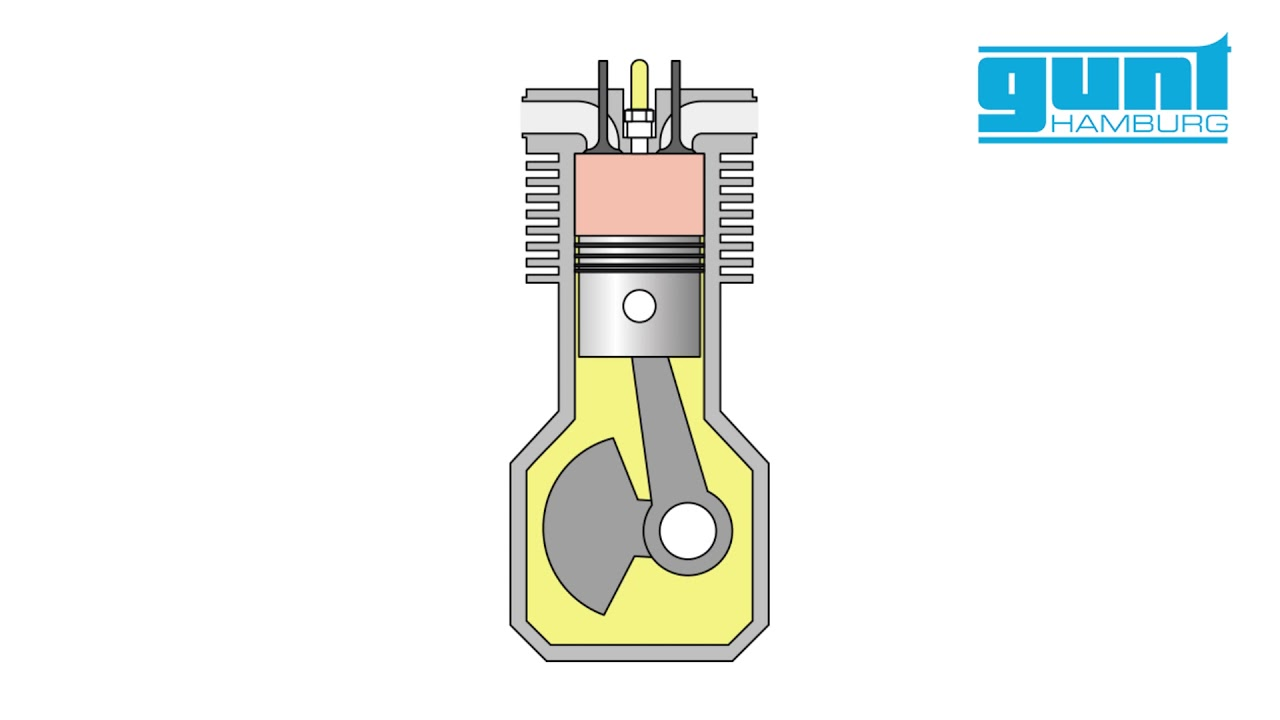
\includegraphics[width=22cm]{nen}};
	%=============================
\end{tikzpicture}
\begin{tikzpicture}[overlay,remember picture,transform shape,>=stealth,line join=round,line cap=round,font=\footnotesize]
	%================================
	\coordinate (A) at (current page.north west);
	\coordinate (B) at (current page.north east);
	\coordinate (C) at (current page.south east);
	\coordinate (D) at (current page.south west);
	\coordinate (AB) at (current page.north);
	\coordinate (CD) at (current page.south);
	\coordinate (AD) at (current page.west);
	\coordinate (BC) at (current page.east);
	\coordinate (G) at (current page.center);
	%================================
	\clip (A) rectangle (C);
	\def\maunen{orange!80} %màu nền cả trang
	\def\mautren{brown!80!black} %màu trên
	\def\mauchu{teal} %màu chữ
		%-- Vẽ các hình cầu trang trí NGẪU NHIÊN
	\coordinate (BB) at ([yshift=2 cm]D);
	\foreach \x in {1,...,20}{
		\pgfmathsetmacro{\r}{abs(random()*0.7)}
		\pgfmathsetmacro{\f}{35*\r)}
		\pgfmathsetmacro{\i}{abs(random()*15)}
		\pgfmathsetmacro{\j}{abs(random()*6)}
		\fill[ball color=green!30,opacity=1] ([xshift=\i cm,yshift=\j cm]BB)  circle (\r);
	}
	
	%=============================TOÁN HỌC
	\coordinate (TT) at ([xshift=0cm,yshift=-3cm]G);
	\coordinate (GG) at ([xshift=-7.65cm,yshift=5.3cm]BC); % điểm đặt chữ
	\def\n{0.75} %độ dày của bóng
	\def\gocnghieng{40} %nghiêng của bóng
	\def\x{5}\def\y{4.9} %co-giãn chữ
	\def\mauchu{red} %màu chữ
	\def\maubong{black}
	\foreach \i in {0,0.01,...,\n}{
		\pgfmathsetmacro\rr{\n-\i}
		\pgfmathsetmacro\domo{100*\i/\n}
		\node[text=\maubong!\domo!white,xscale=\x,yscale=\y,left] at ($(GG)+(\gocnghieng:\rr)$){\fontfamily{qag}\fontsize{20}{0}\selectfont\bfseries VẬT LÝ};
	}
	\node[text=\mauchu,xscale=\x,yscale=\y,left] at (GG) {\fontfamily{qag}\fontsize{20}{0}\selectfont\bfseries VẬT LÝ};
	%--
	%============================= 6
	\coordinate (TAM) at ([xshift=2.8cm,yshift=-0.65cm]GG);
	\fill[brown!70!white] ([xshift=3mm]TAM) circle (2.85cm);	
	\fill[\mautren,draw=white, line width=2pt] (TAM) circle (2.75cm);
	\node[text=white,xscale=6.5,yscale=7.2] at (TAM) {\fontfamily{qag}\fontsize{18}{0}\selectfont\bfseries 12};
	\node[text=blue,scale=1.25] at ([yshift=-3.75cm]TAM) {\fontfamily{put}\fontsize{20}{0}\selectfont\bfseries HỌC KÌ 1};	
	\node[text=red,xscale=1.05,yscale=1.05,left] at ([yshift=-2.45cm,xshift=-6mm]GG) {\fontfamily{qag}\fontsize{20}{0}\selectfont\bfseries THEO CHƯƠNG TRÌNH MỚI};
		%=============================NXB
	\coordinate (NXB) at ([xshift=0cm,yshift=2cm]CD); % điểm đặt chữ
	\coordinate (TL) at ([xshift=0cm,yshift=1cm]CD); % điểm đặt chữ
	\node[text=blue,xscale=1,yscale=1] at (NXB) {\fontfamily{qag}\fontsize{15}{0}\selectfont\bfseries LỚP VẬT LÝ CÔ THẢO - THẦY SANG};
	\node[text=blue,xscale=1,yscale=1] at (TL) {\fontfamily{qag}\fontsize{15}{0}\selectfont\itshape (Tài liệu lưu hành nội bộ)};
\end{tikzpicture}
\end{document}
